\begin{figure}[p]
\centering
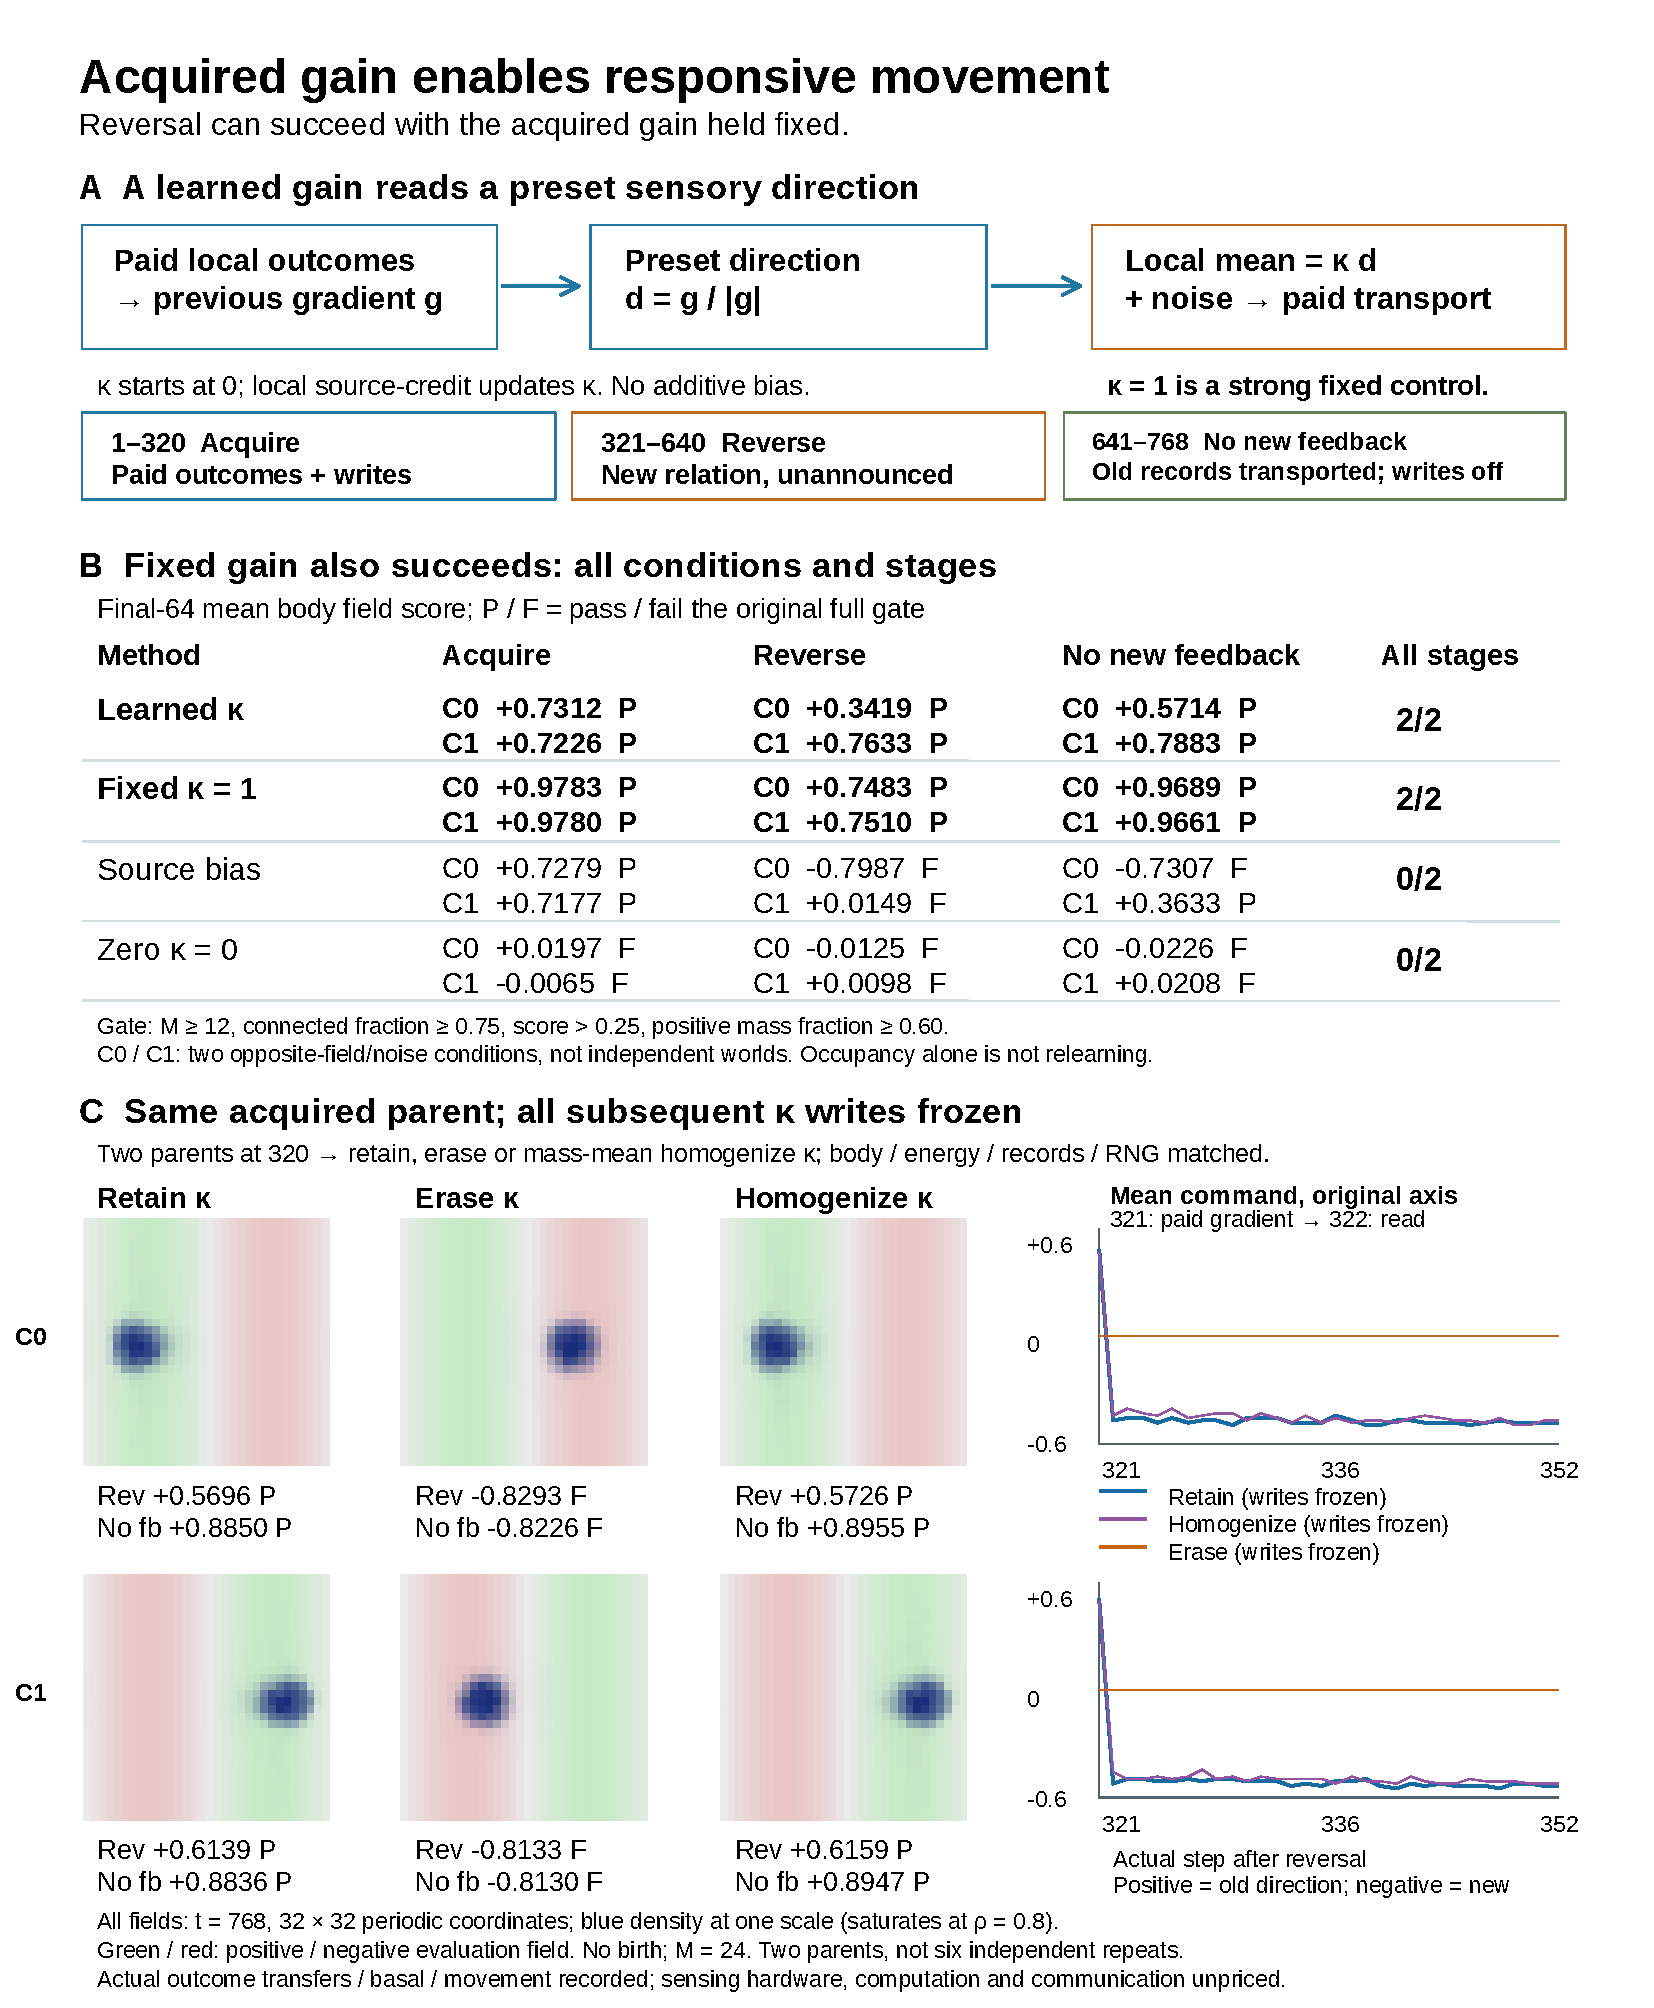
\includegraphics[width=\linewidth,height=0.69\textheight,keepaspectratio]{work/longform_v047/figures/acquired_gain_v0476/acquired_gain.pdf}
\captionsetup{font=footnotesize}
\caption{\textbf{Acquired response gain supports turning without a requirement to relearn the reversal.}
\textbf{a}, A standard local score rule learns an initially zero scalar gain multiplying the direction of a previous actually paid local gradient. Sensory direction and the actuator are supplied. Acquisition and unannounced reversal each last 320 updates; the final 128 add no new payments, observations or writes, while older legal records are transported and read.
\textbf{b}, All four methods and both seed--field conditions retain their final-64 field scores and original composite gates. Learned and fixed positive gain each pass all three phases in both conditions; bias and zero-gain controls do not. Passing the occupancy criterion is not by itself evidence of relearning. Physical costs are reported separately.
\textbf{c}, Two actual acquired parents at 320 supply retained, erased and mass-mean-homogenized gain continuations with gain writing frozen. Retention and homogenization pass both later phases; erasure fails. Curves show the actual mean commands at updates 321--352, not displacement; they change after the new paid observation despite frozen gain. The displayed fields are actual states at update 768 and use original periodic coordinates and a common density scale: blue opacity is $\min(\rho/0.8,1)$, with green/red indicating favourable/unfavourable evaluation fields. Scores under fields describe phase windows, not the displayed snapshot. The six futures are paired interventions from two parents. Homogenization preserves the scalar mean, not each nonlinear action, and global averaging is used only to construct the intervention. All paths remain mass 24 with no tissue birth. Local outcome transfers, basal and movement costs are recorded; computation, communication and sensing hardware have no separate tariff. These results establish a usable acquired response strength, not superiority to fixed positive gain, spatial-pattern necessity, or learning through regeneration.}
\label{fig:acquired-gain}
\end{figure}
